\section{Testing}
To ensure the Parallel Genetic Algorithms implementations are producing expected outcome there is no alternative but to carry out testing. These tests were performed to validate the correctness of PGA implementation. We wanted to see if the output of the PGA program is consistent with the output of original SGA program using same parameters values and random seed.

\subsection{Test Configuration}
\label{test_config}
The common parameter values shown in Table \ref{tbl:test_params} are used for all testing both SGA and PGA programs.

\begin{table}[]
\centering
\caption{Parameters alues used with test cases.}
\label{tbl:test_params}
\begin{tabular}{|l|l|l|}
\hline
\textbf{Parameter}  & \textbf{Description }                        & \textbf{Value}     \\ \hline
POPSIZE    & Population Size                     & 5000      \\ \hline
MAXGENS    & Number of Generation                & 100       \\ \hline
NVARS      & Number of variables in a Chromosome & 3         \\ \hline
PXOVER     & Probability of Crossover            & 0.8       \\ \hline
PMUTATION  & Probability of Mutation             & 0.15      \\ \hline
FITNESS\_F & Fitness function (F8: Griewank)                   & F8        \\ \hline
SEED       & Random value generator seed         & 123456789 \\ \hline
Genome Encoding       & Encoding scheme for genome representaion         & Real value Encoding \\ \hline
\end{tabular}
\end{table}

As the original SGA was implemented with Real-value encoding scheme for genome representation the range of these values are given using a input file. For this test configuration with 3 genome per chromosome the permissible values are given as listed in Table \ref{tbl:genome_range}.

\begin{table}[]
\centering
\caption{Genome value range for 3 variables Griewank function}
\label{tbl:genome_range}
\begin{tabular}{|l|l|}
\hline
\textbf{Lower} & \textbf{Upper} \\ \hline
-512.0           & 511.0            \\ \hline
-512.0           & 511.0            \\ \hline
-512.0           & 511.0            \\ \hline
\end{tabular}
\end{table}

As discussed in section \ref{beowulf:process_manager} the hosts information entries shown in Listing \ref{lst:config_hydra} were added for Hydra (MPI Process Manager). The entry at line 1 is master node's hostname. Which means master node also is acting as a compute node in the cluster.

\begin{lstlisting}[style=BashInputStyle, label={lst:config_hydra}, caption={The hosts file configuration for Hydra.}]
padma:2
meghna:2
jamuna:2
\end{lstlisting} 

The PGA program was run by using following command:
\begin{lstlisting}[style=BashInputStyle, label={lst:run_mpi}]
$mpiexec -f ~/hosts -n 6 ./pga
\end{lstlisting}
The command \textbf{mpiexec} takes in parameter \textbf{-f} for the hosts file name and \textbf{-n} for  the number of processes that needs to be created in the cluster. The example shown above will launch 6 process that will run the executable binary \textbf{pga}.

\textbf{All tests results shown in this section are carried out in Hardware based Beowulf} system not in simulated cluster.

\subsection{Tests Outcome}
The GA programs output for the SGA, PGA v1, PGA v2 and PGA v3 are shown below. As these tests were run with a generation size if 100 the full output is not shown to save space. Instead, outputs are shown into two split images "Top part" and "Bottom part" of the screen capture that convey most important information. We are assuming the original SGA program is producing a correct output. Then the subsequent 3 PGA programs outputs are compared against SGA's output to validate and analyse each PGA implementation. 

\subsubsection{SGA Output}

Figures \ref{fig:test_sga_top} and \ref{fig:test_sga_bottom} shows the output of original SGA program compiled with the parameter configuration discussed in section \ref{test_config}.

\begin{figure}[!htb]
	\center
        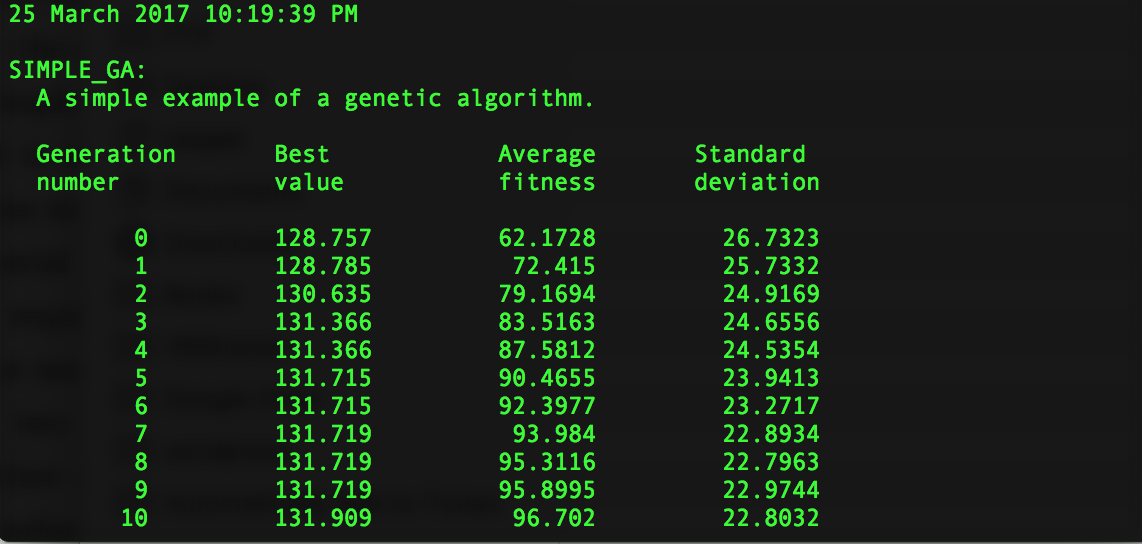
\includegraphics[width= \linewidth]{figs/tests/sga_top.png}
    \caption{SGA output - Top part}
     \label{fig:test_sga_top}
\end{figure}

\begin{figure}[!htb]
	\center
        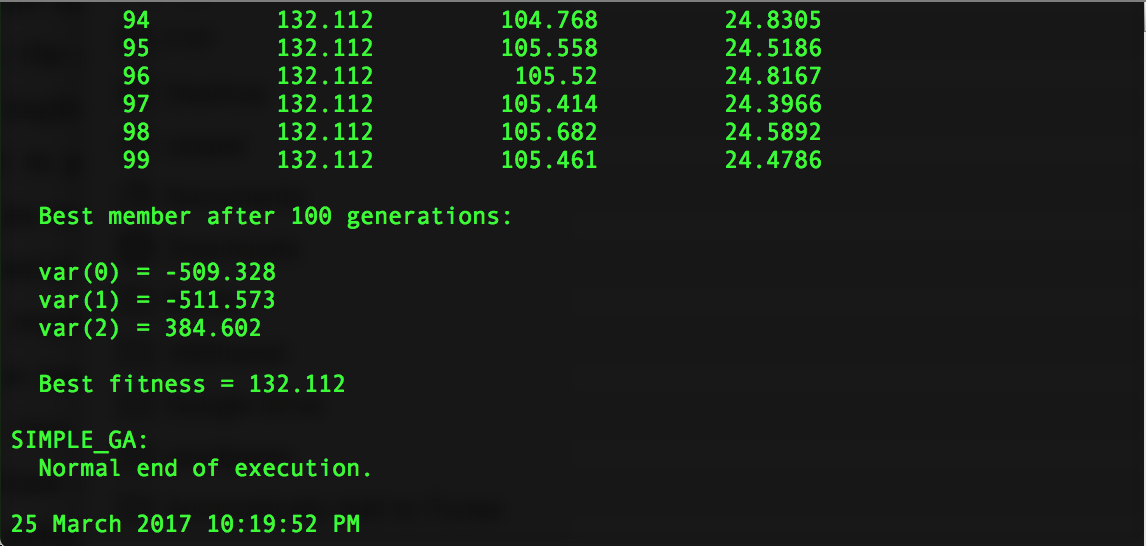
\includegraphics[width= \linewidth]{figs/tests/sga_bottom.png}
    \caption{SGA output - Bottom part}
     \label{fig:test_sga_bottom}
\end{figure}

\subsubsection{PGA v1 Output}

Figures \ref{fig:test_pga_top} and \ref{fig:test_pga_bottom} shows the output of original PGA v1 compiled with the parameter configuration discussed in section \ref{test_config}.

\begin{figure}[!htb]
	\center
        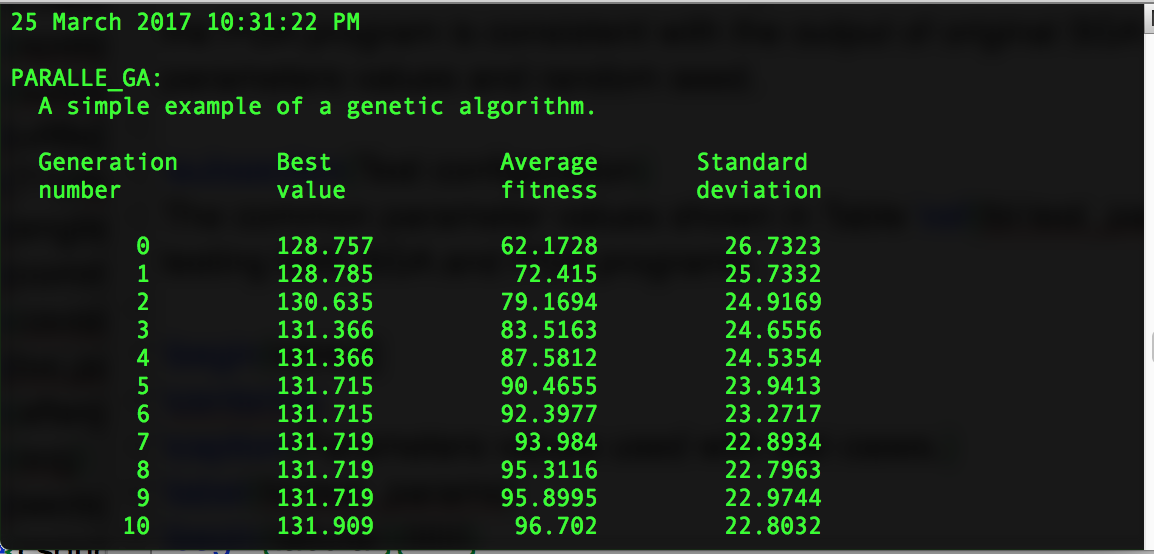
\includegraphics[width= \linewidth]{figs/tests/pga_top.png}
    \caption{PGA v1 output - Top part}
     \label{fig:test_pga_top}
\end{figure}

\begin{figure}[!htb]
	\center
        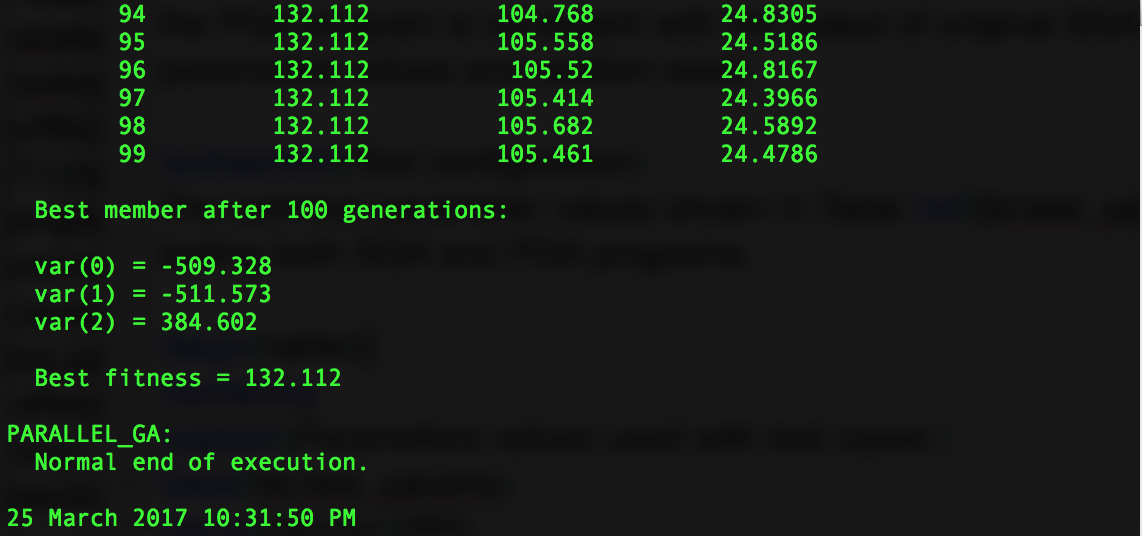
\includegraphics[width= \linewidth]{figs/tests/pga_bottom.png}
    \caption{PGA v2 output - Bottom part}
     \label{fig:test_pga_bottom}
\end{figure}

\subsubsection{PGA v2 Output}

Figures \ref{fig:test_pgav2_top} and \ref{fig:test_pgav2_bottom} shows the output of original PGA v2 compiled with the parameter configuration discussed in section \ref{test_config}.

\begin{figure}[!htb]
	\center
        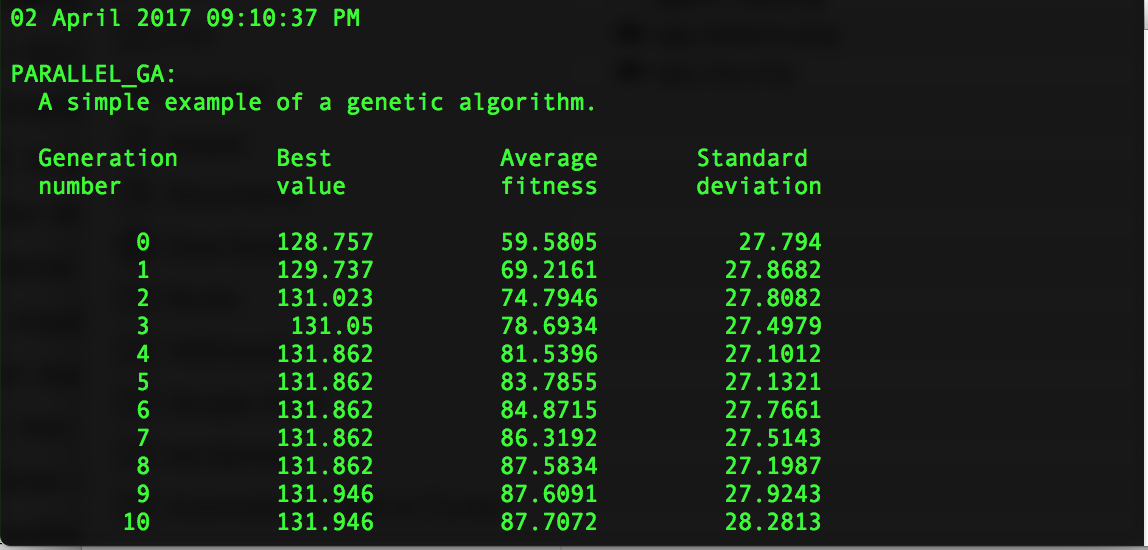
\includegraphics[width= \linewidth]{figs/tests/pgav2_top.png}
    \caption{PGA v1 output - Top part}
     \label{fig:test_pgav2_top}
\end{figure}

\begin{figure}[!htb]
	\center
        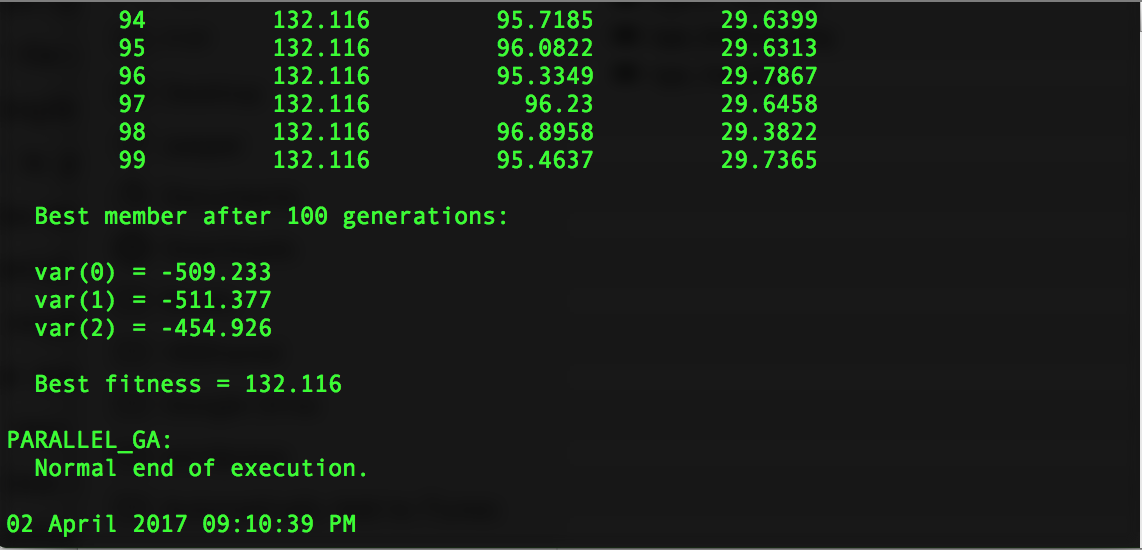
\includegraphics[width= \linewidth]{figs/tests/pgav2_bottom.png}
    \caption{PGA v2 output - Bottom part}
     \label{fig:test_pgav2_bottom}
\end{figure}

\subsubsection{PGA v3 Output}

Figures \ref{fig:test_pgav3_top} and \ref{fig:test_pgav3_bottom} shows the output of original PGA v3 compiled with the parameter configuration discussed in section \ref{test_config}.

\begin{figure}[!htb]
	\center
        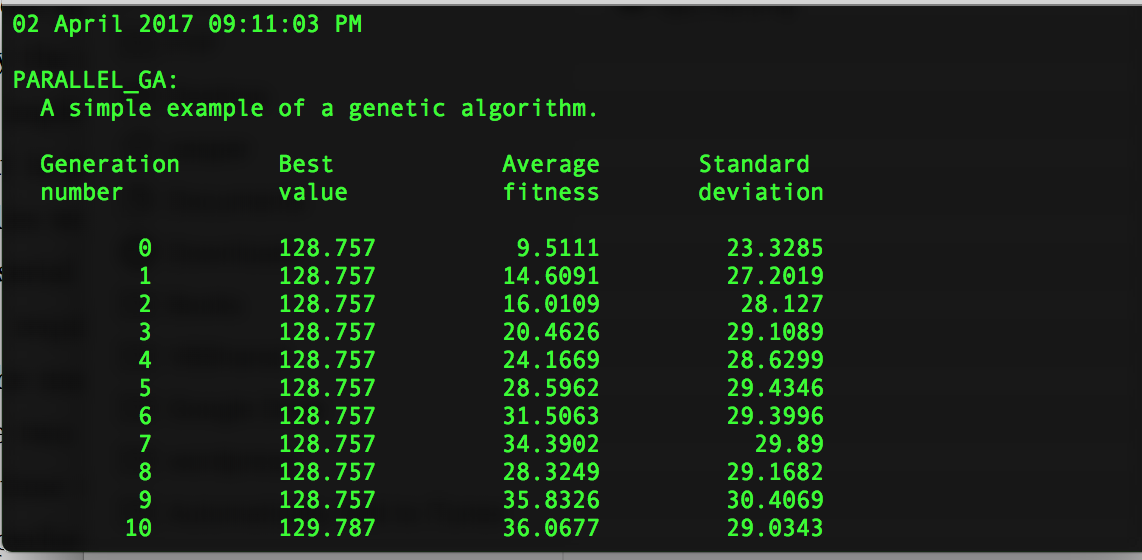
\includegraphics[width= \linewidth]{figs/tests/pgav3_top.png}
    \caption{PGA v3 output - Top part}
     \label{fig:test_pgav3_top}
\end{figure}

\begin{figure}[!htb]
	\center
        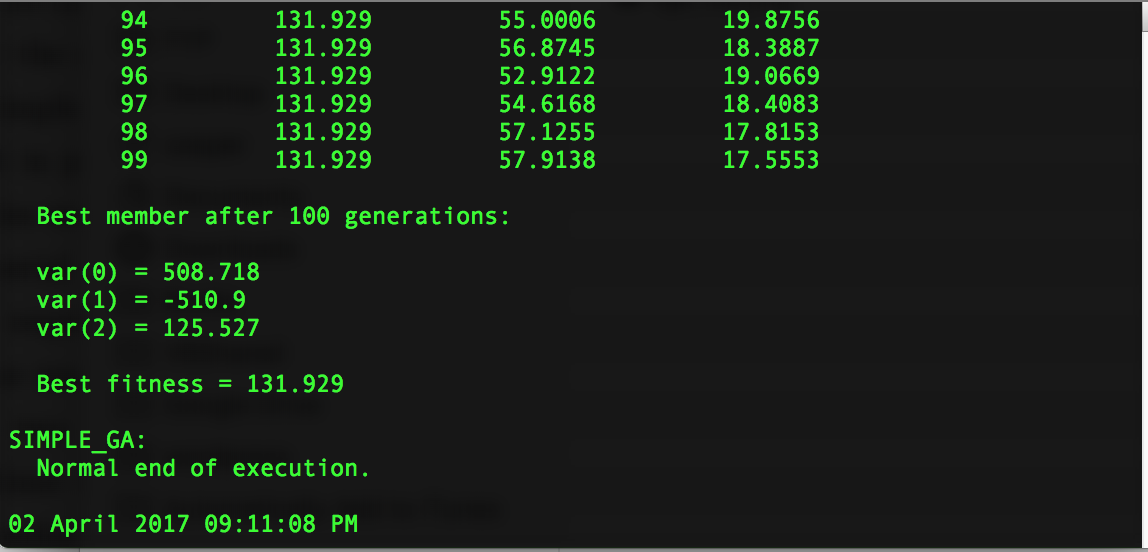
\includegraphics[width= \linewidth]{figs/tests/pgav3_bottom.png}
    \caption{PGA v3 output - Bottom part}
     \label{fig:test_pgav3_bottom}
\end{figure}

 

